%% Expanded IEEE journal-style sample paper (~15-20 pages when compiled).
%% Compile: pdflatex ieee_paper.tex  (twice)
\documentclass[journal]{IEEEtran}
\usepackage{cite}
\usepackage{amsmath,amssymb,amsfonts}
\usepackage{algorithm}
\usepackage{algpseudocode}
\usepackage{graphicx}
\usepackage{textcomp}
\usepackage{xcolor}
\usepackage{booktabs}
\usepackage{multirow}
\usepackage{tabularx}
\usepackage{url}
\usepackage{hyperref}
\usepackage{bm}

\graphicspath{{figures/}}

\begin{document}

\title{Federated Averaging for Multi-Class Network Intrusion Classification:\\
Theoretical Foundations, Empirical Evaluation, and Resilience to Label Poisoning\\
on the CIC--UNSW-NB15 Dataset}

\author{
\IEEEauthorblockN{Jay Mehta}
\IEEEauthorblockA{
\textit{Independent Research / Academic Project}\\
Corresponding author e-mail: (author contact)
}
}

\maketitle

\begin{abstract}
Federated learning (FL) enables multiple institutions to jointly train machine learning models without exchanging raw data, a property that is especially desirable for network security analytics where flow telemetry may contain sensitive operational information. This paper presents a comprehensive theoretical and empirical study of Federated Averaging (FedAvg) applied to multi-class intrusion / traffic classification on the CIC--UNSW-NB15 augmented dataset. We formalize the FL objective, the FedAvg update rule, local empirical risk minimization with multilayer perceptrons (MLPs), and a single-client label-poisoning threat model. We then conduct a 64-configuration experimental sweep over client counts, global communication rounds, local epochs, and poison intensities. Empirically, longer training improves clean accuracy (best clean accuracy $\approx 0.924$), while targeted poisoning is most harmful when a single client dominates training (worst accuracy $\approx 0.856$). With multiple clients, FedAvg dilutes one poisoned shard and accuracy typically remains above $0.90$. Confusion-matrix and one-vs-rest TP/FP/FN/TN analyses show that majority-class targeted poisoning systematically increases false positives for class~0 and reduces recall for several minority attack categories---an effect that can be understated by overall accuracy alone under severe class imbalance. We discuss communication cost, convergence intuition under IID shards, limitations of the simulation setting, and directions for robust aggregation. An interactive dashboard accompanies the study for transparent inspection of all runs.
\end{abstract}

\begin{IEEEkeywords}
Federated learning, Federated Averaging (FedAvg), intrusion detection systems, network traffic classification, data poisoning, label flipping, CIC--UNSW-NB15, multilayer perceptron, confusion matrix, class imbalance
\end{IEEEkeywords}

\section{Introduction}

\subsection{Motivation}
Network intrusion detection and traffic classification increasingly rely on supervised learning over high-dimensional flow features. In operational settings, however, the organizations that collect such telemetry---enterprises, internet service providers, campus networks, or industrial control environments---are often unwilling or legally unable to centralize raw records. Privacy regulations, competitive sensitivity, and breach-risk all discourage naive data pooling.

Federated learning~\cite{mcmahan2017communication,kairouz2021advances} offers an alternative: each participant trains on local data and shares only model parameters (or gradients), which a coordinating server aggregates into a global model. For intrusion detection, this paradigm suggests a path toward collaborative detection quality without collaborative data warehouses~\cite{rahman2020internet}.

\subsection{Problem Statement}
We study the following concrete problem. Given a tabular multi-class dataset with feature vectors $\mathbf{x}\in\mathbb{R}^{d}$ and labels $y\in\{0,\ldots,C-1\}$, simulate $N$ clients holding disjoint training shards and learn a shared classifier $f_{\theta}$ via FedAvg. We then ask:
\begin{enumerate}
\item How do $N$, the number of global rounds $R$, and local epochs $E$ affect test accuracy and F1-score?
\item How does label poisoning on a single client, with fraction $f$ of labels corrupted, change global performance?
\item Does poisoning alter \emph{which} classes are confused, beyond aggregate metrics?
\end{enumerate}

\subsection{Scope and Simulation Nature}
All experiments in this repository run on a single machine. ``Clients'' are logical partitions of a shuffled training set rather than physically distributed hosts. The simulation preserves the algorithmic structure of FL (local optimization + server aggregation) while abstracting away network latency, dropouts, and systems engineering. This is appropriate for controlled scientific comparison of learning dynamics and poisoning effects, but it is not a full systems deployment study.

\subsection{Contributions}
\begin{enumerate}
\item A self-contained theoretical presentation of FedAvg for multi-class classification, including the global objective, local surrogate losses, weighted aggregation, and a formal label-poisoning adversary.
\item An end-to-end reproducible pipeline on CIC--UNSW-NB15 augmented data: cleaning, stratified splitting, scaling, IID sharding, MLP training, and evaluation with confusion matrices and per-class TP/FP/FN/TN.
\item A 64-run experimental grid quantifying interactions among clients, rounds, local epochs, and poison settings, with best-case clean accuracy near $0.924$ and worst-case poisoned accuracy near $0.856$.
\item Qualitative and quantitative evidence that majority-class targeted poisoning induces a ``predict class~0 when uncertain'' bias that is most severe under single-client training and largely diluted under multi-client FedAvg.
\item Public interactive visualizations of the full experimental record.
\end{enumerate}

\subsection{Paper Organization}
Section~\ref{sec:background} reviews FL, IDS learning, and poisoning. Section~\ref{sec:theory} develops the mathematical framework. Section~\ref{sec:method} describes the system design. Section~\ref{sec:setup} details the experimental protocol. Sections~\ref{sec:results}--\ref{sec:discussion} present and interpret results. Section~\ref{sec:conclusion} concludes.

\section{Background and Related Work}
\label{sec:background}

\subsection{Centralized Learning for Intrusion Detection}
Classical machine learning for IDS ranges from shallow models (decision trees, SVMs, random forests) to deep neural networks trained on packet or flow features. Centralized training assumes a single data lake. While often accurate in benchmarks, this assumption conflicts with multi-organization collaboration. Moreover, network data are characteristically \emph{imbalanced}: benign or majority classes dominate, so accuracy can be misleading unless accompanied by per-class analysis.

\subsection{Federated Learning Basics}
In cross-silo or cross-device FL, a server coordinates rounds of local training and aggregation~\cite{kairouz2021advances}. FedAvg~\cite{mcmahan2017communication} is the canonical algorithm: clients run multiple local SGD/Adam steps and return updated weights; the server averages them, typically weighted by local dataset sizes. Variants address non-IID data (FedProx, SCAFFOLD), communication compression, personalization, and robust aggregation.

\subsection{FL for Security Analytics}
Prior work has explored FL for IoT and network intrusion detection to keep telemetry local while improving collective detectors~\cite{rahman2020internet}. Our contribution is not a new FL optimizer; rather, we provide a carefully instrumented FedAvg case study with poisoning analysis and confusion-level diagnostics on a widely used tabular intrusion dataset.

\subsection{Poisoning and Byzantine Behavior}
Data poisoning injects corrupted training examples to degrade or redirect a learned model. In FL, a malicious client can poison labels or features, or upload crafted weights~\cite{bagdasaryan2020backdoor,tolpegin2020data}. Defenses include robust aggregators (coordinate-wise median, trimmed mean, Krum), anomaly detection on updates, and differential privacy. This paper evaluates \emph{undefended} FedAvg against a simple but realistic label-flipping adversary on one client, establishing an empirical baseline for how much ``natural dilution'' multi-client averaging provides.

\subsection{UNSW-NB15 Family of Datasets}
UNSW-NB15 and related CIC-augmented releases provide labeled flow features covering multiple attack categories alongside normal traffic. We use an augmented CIC--UNSW-NB15 tabular release with $d=76$ numeric features and $C=10$ classes. Exact semantic names of minority classes are less critical for our algorithmic conclusions than the empirical imbalance pattern: one dominant class and several rare classes with near-zero recall under a simple MLP.

\section{Theoretical Framework}
\label{sec:theory}

\subsection{Supervised Multi-Class Risk}
Let $\mathcal{D}$ be a distribution over $\mathcal{X}\times\mathcal{Y}$ with $\mathcal{Y}=\{0,\ldots,C-1\}$. A parametric model $f_{\theta}:\mathcal{X}\to\mathbb{R}^{C}$ produces logits; predicted label is $\hat{y}=\arg\max_{c} [f_{\theta}(\mathbf{x})]_{c}$. The population risk under cross-entropy is
\begin{equation}
\label{eq:risk}
R(\theta) = \mathbb{E}_{(\mathbf{x},y)\sim\mathcal{D}} \Big[ \ell\big(f_{\theta}(\mathbf{x}), y\big) \Big],
\end{equation}
where $\ell(\mathbf{z},y)=-\log\frac{e^{z_y}}{\sum_{c}e^{z_c}}$.

Given a finite training set $S=\{(\mathbf{x}_i,y_i)\}_{i=1}^{n}$, the empirical risk is
\begin{equation}
\hat{R}_S(\theta)=\frac{1}{n}\sum_{i=1}^{n}\ell\big(f_{\theta}(\mathbf{x}_i),y_i\big).
\end{equation}

\subsection{Federated Partition of the Empirical Risk}
Partition $S$ into $N$ disjoint client datasets $S_k$ with $n_k=|S_k|$ and $\sum_k n_k=n$. The global empirical risk decomposes exactly as a mixture of local empirical risks:
\begin{equation}
\label{eq:decomp}
\hat{R}_S(\theta)=\sum_{k=1}^{N} \frac{n_k}{n}\,\hat{R}_{S_k}(\theta).
\end{equation}
Equation~\eqref{eq:decomp} is the conceptual justification for size-weighted FedAvg: averaging models trained on local risks approximates minimizing a weighted combination of those risks when local updates are not too far from the broadcast initialization.

\subsection{Local Optimization}
In round $t$, client $k$ receives $\theta^{t}$ and approximately solves
\begin{equation}
\theta_k^{t+1} \approx \arg\min_{\theta} \hat{R}_{S_k}(\theta)
\quad\text{initialized at }\theta^{t},
\end{equation}
using $E$ epochs of minibatch Adam with learning rate $\eta$. Let $B$ be the minibatch size. The number of local gradient steps per round is roughly $E\cdot\lceil n_k/B\rceil$. More local steps increase client drift away from $\theta^{t}$ but also increase local progress per communication round---the classic FedAvg trade-off.

\subsection{FedAvg Aggregation}
The server sets
\begin{equation}
\label{eq:fedavg}
\theta^{t+1}=\sum_{k=1}^{N} w_k\,\theta_k^{t+1},
\qquad
w_k=\frac{n_k}{\sum_{j=1}^{N}n_j}.
\end{equation}
If shards are equal-sized, $w_k=1/N$. Aggregation is performed element-wise over all tensors in the state dictionary (weights and biases of every layer).

\subsection{Communication Cost Model}
Let $|\theta|$ denote the number of scalar parameters. Each round transmits approximately $N|\theta|$ parameters uplink and $N|\theta|$ downlink (broadcast counted per client), i.e., $\Theta(N|\theta|)$ communication per round. Total communication over $R$ rounds scales as $\Theta(R N |\theta|)$. Increasing $E$ reduces required $R$ for a target accuracy in many IID settings, improving communication efficiency---one of FedAvg's original motivations~\cite{mcmahan2017communication}.

\subsection{MLP Hypothesis Class}
Our model is a two-hidden-layer MLP:
\begin{equation}
f_{\theta}(\mathbf{x})=W_3\,\sigma\big(W_2\,\sigma(W_1\mathbf{x}+b_1)+b_2\big)+b_3,
\end{equation}
with $\sigma=\mathrm{ReLU}$, hidden width $128$, $d=76$, and $C=10$. The hypothesis class is rich enough for nonlinear decision boundaries on tabular features, yet small enough for rapid experimentation. Softmax is implicit in the cross-entropy loss.

\subsection{Class Imbalance and Metrics}
Let $n^{(c)}$ be the number of test examples of class $c$. Overall accuracy is
\begin{equation}
\mathrm{Acc}=\frac{1}{n_{\mathrm{test}}}\sum_{i=1}^{n_{\mathrm{test}}}\mathbf{1}[\hat{y}_i=y_i].
\end{equation}
Under imbalance, $\mathrm{Acc}$ is dominated by majority-class correctness. We therefore also report precision, recall, F1 (from scikit-learn's classification report aggregates), the full confusion matrix $M\in\mathbb{N}^{C\times C}$ with
\begin{equation}
M_{ij}=\#\{i': y_{i'}=i,\ \hat{y}_{i'}=j\},
\end{equation}
and one-vs-rest counts
\begin{align}
\mathrm{TP}_c&=M_{cc},\\
\mathrm{FP}_c&=\sum_{i\neq c}M_{ic},\\
\mathrm{FN}_c&=\sum_{j\neq c}M_{cj},\\
\mathrm{TN}_c&=n_{\mathrm{test}}-\mathrm{TP}_c-\mathrm{FP}_c-\mathrm{FN}_c.
\end{align}
Per-class recall $\mathrm{TP}_c/(\mathrm{TP}_c+\mathrm{FN}_c)$ is especially informative for rare attacks.

\subsection{Threat Model: Label Poisoning}
\label{sec:threat}
We consider a dirty-label adversary controlling client $0$ only. Features remain untouched; a fraction $f\in[0,1]$ of local labels are replaced according to a mode $m$:
\begin{itemize}
\item \textbf{Target:} $y\leftarrow y_{\mathrm{tgt}}$ (we use $y_{\mathrm{tgt}}=0$).
\item \textbf{Random-wrong:} $y\leftarrow$ uniform over $\mathcal{Y}\setminus\{y_{\mathrm{true}}\}$.
\item \textbf{Cycle:} $y\leftarrow (y+1)\bmod C$.
\end{itemize}
The adversary does not modify uploaded weights beyond ordinary training on poisoned labels, and does not control the test distribution. This models a compromised or negligent data pipeline at one silo rather than an optimal model-replacement attack~\cite{bagdasaryan2020backdoor}.

\subsection{Why Dilution Occurs under FedAvg}
Suppose equal shard sizes and one poisoned client. Even if $\theta_0^{t+1}$ is strongly biased, the aggregate is
\begin{equation}
\theta^{t+1}=\frac{1}{N}\theta_0^{t+1}+\frac{1}{N}\sum_{k=1}^{N-1}\theta_k^{t+1}.
\end{equation}
As $N$ grows, the poisoned update's coefficient $1/N$ shrinks. This is not a cryptographic defense and fails if many clients collude or if the adversary mounts stronger model poisoning; but it explains our empirical observation that multi-client runs remain near clean accuracy under single-client label flips.

\subsection{Convergence Intuition (IID Case)}
When shards are IID draws from the same distribution, local risks $\hat{R}_{S_k}$ are statistically similar. Local Adam steps from a shared initialization tend to move in related directions, so averaging is constructive. Formal FedAvg convergence bounds typically assume smoothness, bounded variance, and control of client drift as a function of $E$ and heterogeneity~\cite{kairouz2021advances}. Our shards are IID-like by construction (random shuffle then cut), placing us near the favorable regime. Non-IID partitions would increase drift and could amplify poisoning or reduce clean accuracy; we leave that to future work.

\section{System Design and Implementation}
\label{sec:method}

\subsection{Data Pipeline}
Figure~\ref{fig:pipeline} summarizes preprocessing. Features and labels are aligned row-wise. Non-finite values are replaced by zeros. A stratified split (default $80\%$ train / $20\%$ test) preserves class proportions. A \texttt{StandardScaler} is fit on training features only, then applied to train and test. Training indices are shuffled with a fixed seed and split into $N$ contiguous shards after permutation.

\begin{figure}[!t]
\centering
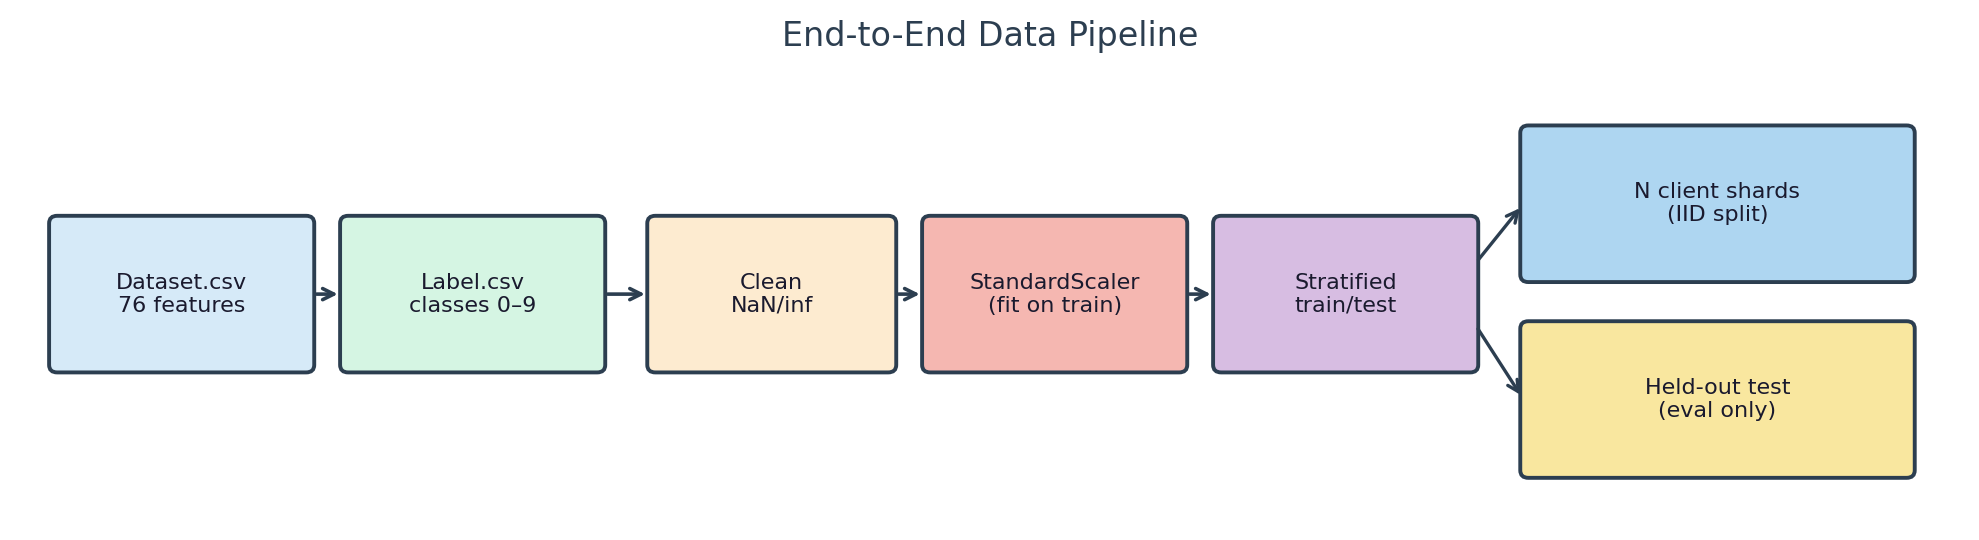
\includegraphics[width=\columnwidth]{fig_pipeline.png}
\caption{End-to-end data pipeline from raw CSVs to client shards and a held-out test set.}
\label{fig:pipeline}
\end{figure}

\paragraph{Note on global scaling.}
Fitting a scaler on pooled training features is a practical simplification for a single-machine simulation. Strictly decentralized FL might estimate normalization statistics via secure aggregation or use per-client normalization. We explicitly document this assumption.

\subsection{Model Architecture}
Figure~\ref{fig:mlp} shows the shared MLP. Identical architecture across clients is mandatory for element-wise FedAvg.

\begin{figure}[!t]
\centering
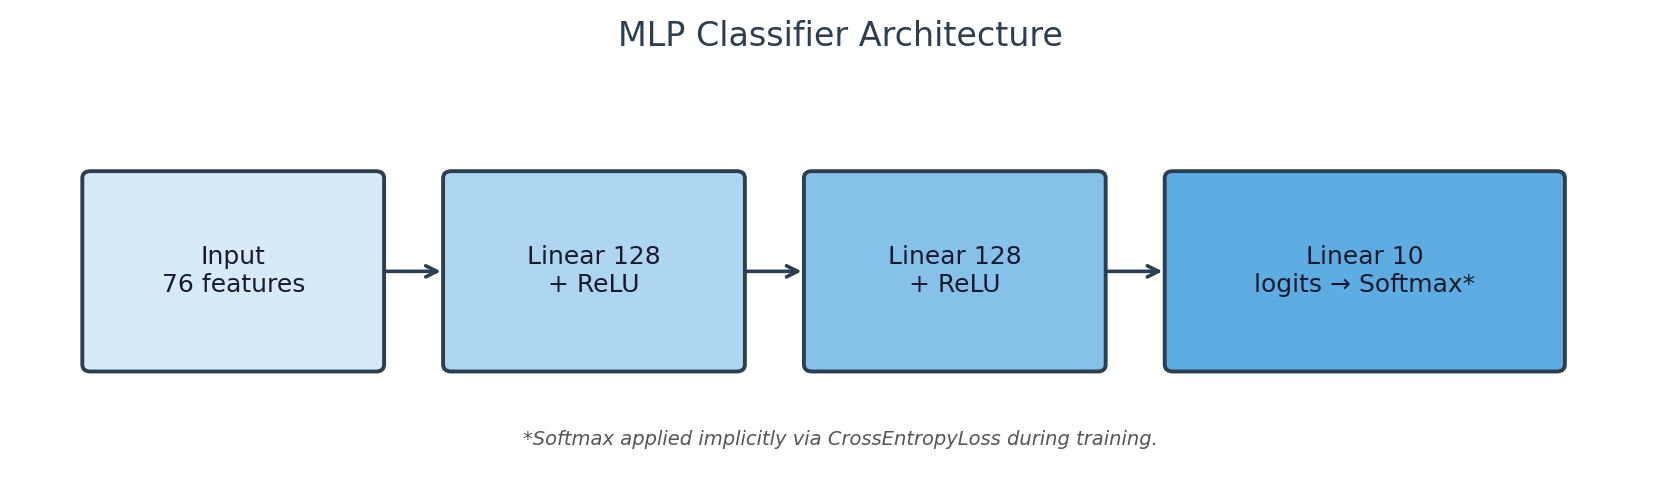
\includegraphics[width=\columnwidth]{fig_mlp.png}
\caption{Shared MLP classifier used by every client.}
\label{fig:mlp}
\end{figure}

\subsection{Federated Training Loop}
Figure~\ref{fig:fedavg} and Algorithm~\ref{alg:fedavg} describe one round of training.

\begin{figure}[!t]
\centering
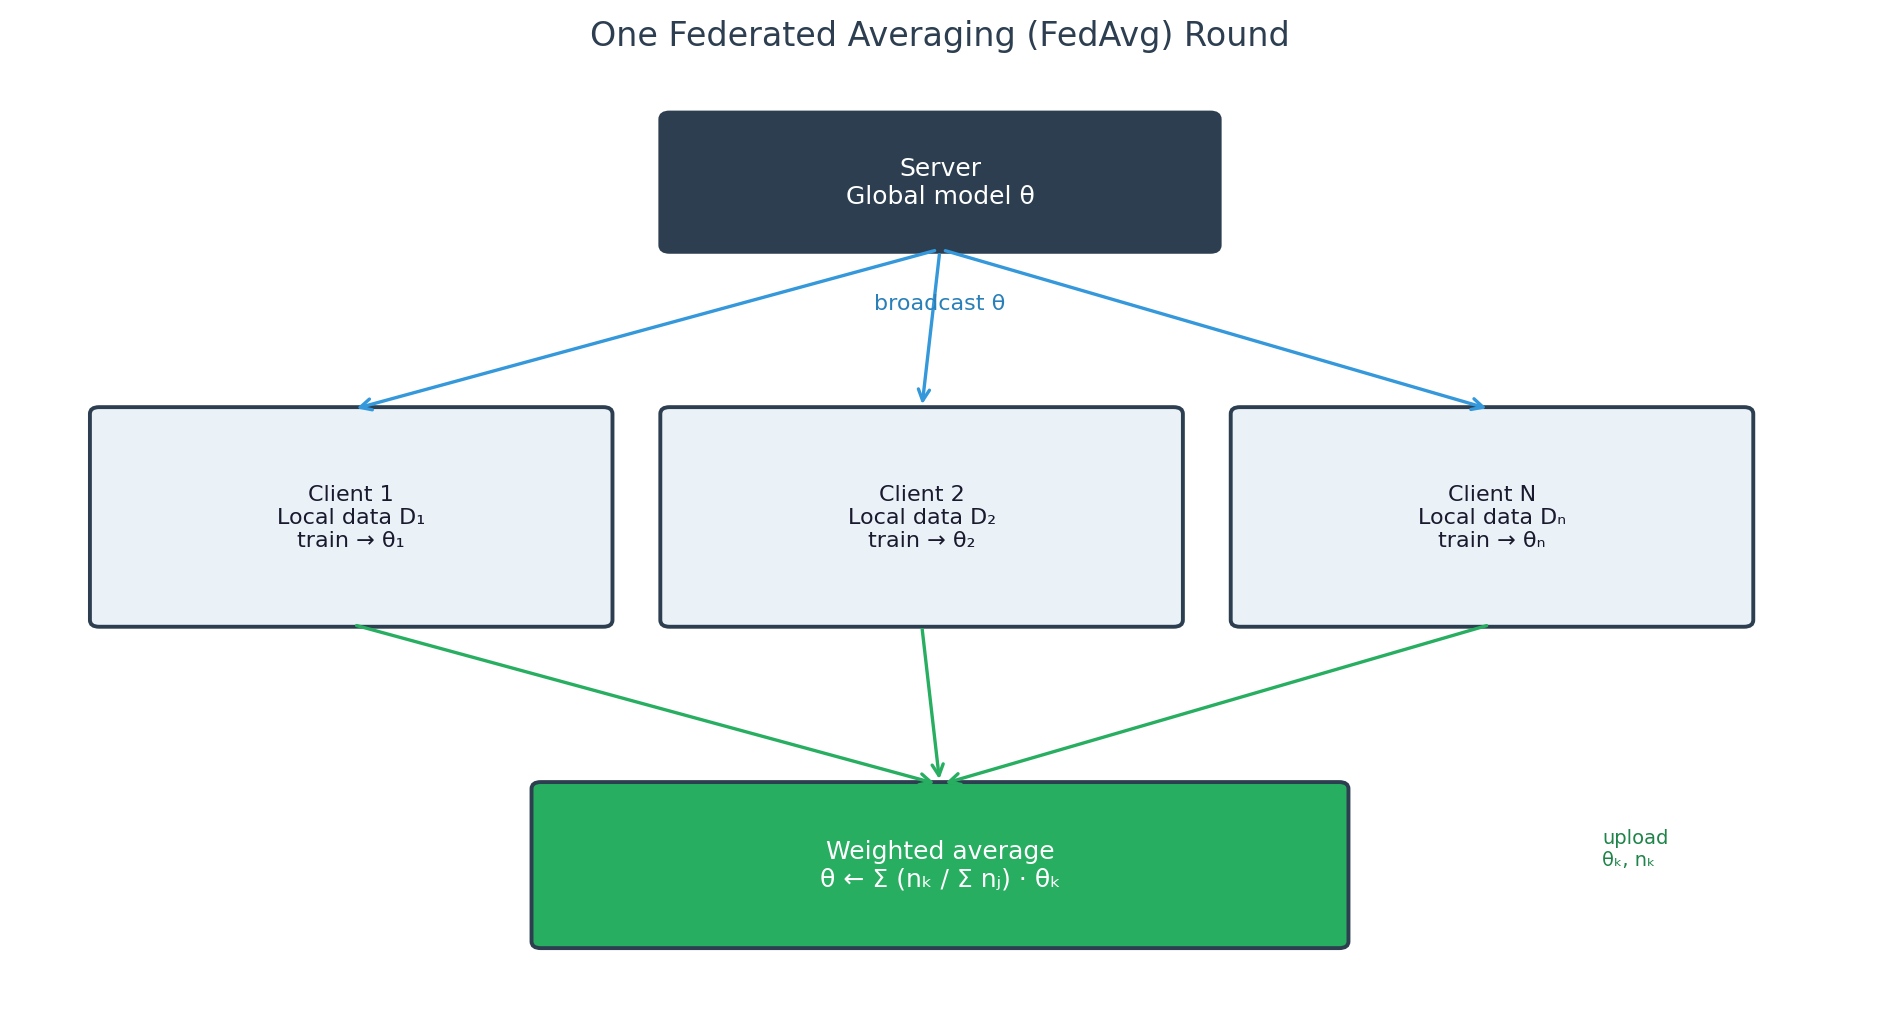
\includegraphics[width=\columnwidth]{fig_fedavg.png}
\caption{One FedAvg round: broadcast, local training, and weighted aggregation.}
\label{fig:fedavg}
\end{figure}

\begin{algorithm}[t]
\caption{FedAvg for intrusion classification (simulation)}
\label{alg:fedavg}
\begin{algorithmic}[1]
\Require clients $\{S_k\}_{k=1}^{N}$, rounds $R$, local epochs $E$, batch size $B$, learning rate $\eta$
\State initialize global model $\theta^{0}$
\For{$t=0$ to $R-1$}
  \For{each client $k=1,\ldots,N$ \textbf{in parallel}}
    \State $\theta_k \leftarrow \theta^{t}$
    \For{$e=1$ to $E$}
      \For{each minibatch $\mathcal{B}\subset S_k$}
        \State Adam update on $\hat{R}_{\mathcal{B}}(\theta_k)$ with step $\eta$
      \EndFor
    \EndFor
    \State upload $(\theta_k, n_k)$
  \EndFor
  \State $\theta^{t+1}\leftarrow\sum_k (n_k/\sum_j n_j)\,\theta_k$
  \State evaluate $\theta^{t+1}$ on held-out test set
\EndFor
\State \Return $\theta^{R}$
\end{algorithmic}
\end{algorithm}

\subsection{Poisoning Hook}
Before local training begins, if poisoning is enabled, client~$0$'s label vector is rewritten according to Section~\ref{sec:threat} (Fig.~\ref{fig:poison}). Features and all other clients remain clean.

\begin{figure}[!t]
\centering
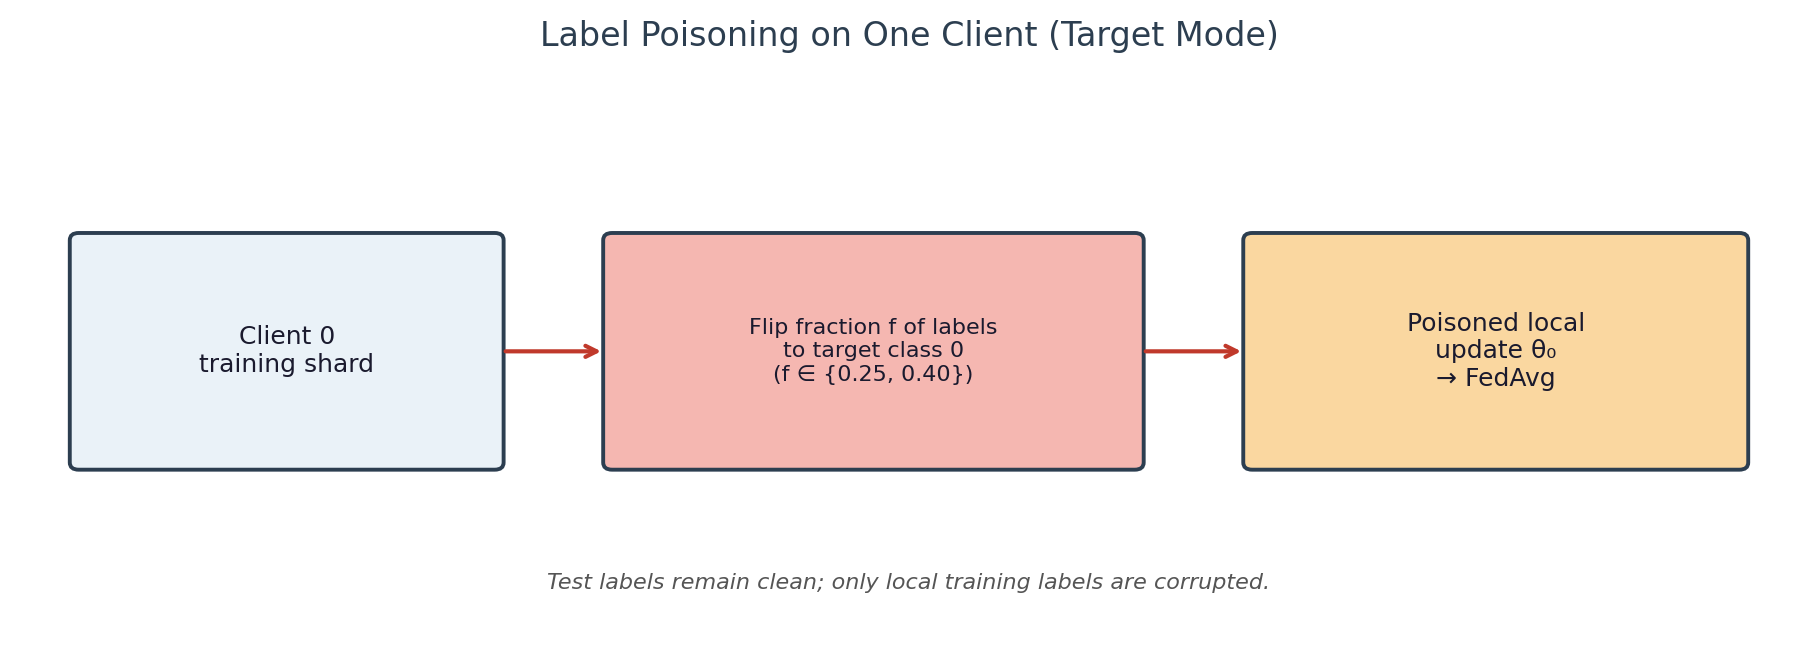
\includegraphics[width=0.95\columnwidth]{fig_poison.png}
\caption{Targeted label poisoning applied only to client~0 training labels.}
\label{fig:poison}
\end{figure}

\subsection{Software Stack}
The implementation uses PyTorch for the MLP and optimization, pandas/NumPy for data loading, and scikit-learn for splitting, scaling, confusion matrices, and classification reports. Experiments are driven by a configuration dataclass and CLI flags for clients, rounds, local epochs, batch size, learning rate, device, and poison parameters.

\section{Experimental Setup}
\label{sec:setup}

\subsection{Hardware and Reproducibility}
Runs use CPU by default with fixed random seeds for NumPy and PyTorch. This favors reproducibility over wall-clock speed.

\subsection{Grid Design}
The principal sweep comprises 64 configurations exploring:
\begin{itemize}
\item $N\in\{1,2,3,5\}$,
\item global rounds (notably $5$ and $10$ in the grid),
\item local epochs $E\in\{1,2\}$,
\item poison fraction $f\in\{0,0.25,0.40\}$,
\item poison mode $\in\{\mathrm{target},\mathrm{random\_wrong}\}$ when $f>0$.
\end{itemize}
Primary metrics: test accuracy, precision, recall, F1. Selected representative scenarios additionally store full confusion matrices.

\subsection{Descriptive Statistics of the Sweep}
Across all 64 runs, accuracy has mean $\approx 0.907$, standard deviation $\approx 0.014$, minimum $\approx 0.856$, and maximum $\approx 0.924$. The relatively small standard deviation indicates that most configurations remain in a high-accuracy band; the lower tail is concentrated in heavily poisoned single-client settings.

\subsection{Evaluation Protocol}
The test set is never poisoned and never used for training. After the final round (and optionally intermediate rounds), we compute aggregate metrics and, for key scenarios, confusion matrices and TP/FP/FN/TN.

\subsection{Artifacts}
Results are exported to CSV; static figures and an interactive HTML dashboard summarize the sweep. The live dashboard is available at \url{https://fl-research.vercel.app}.

\section{Results}
\label{sec:results}

\subsection{Clean Training Behavior}
Under clean labels, increasing $R$ and $E$ generally improves accuracy. Single-client clean training can slightly outperform multi-client FedAvg at the same budget because there is no averaging-induced damping of local specialization; however, multi-client accuracy remains strong (typically $>0.90$). Figures~\ref{fig:rounds} and~\ref{fig:local_epochs} illustrate round and local-epoch effects.

\begin{figure}[!t]
\centering
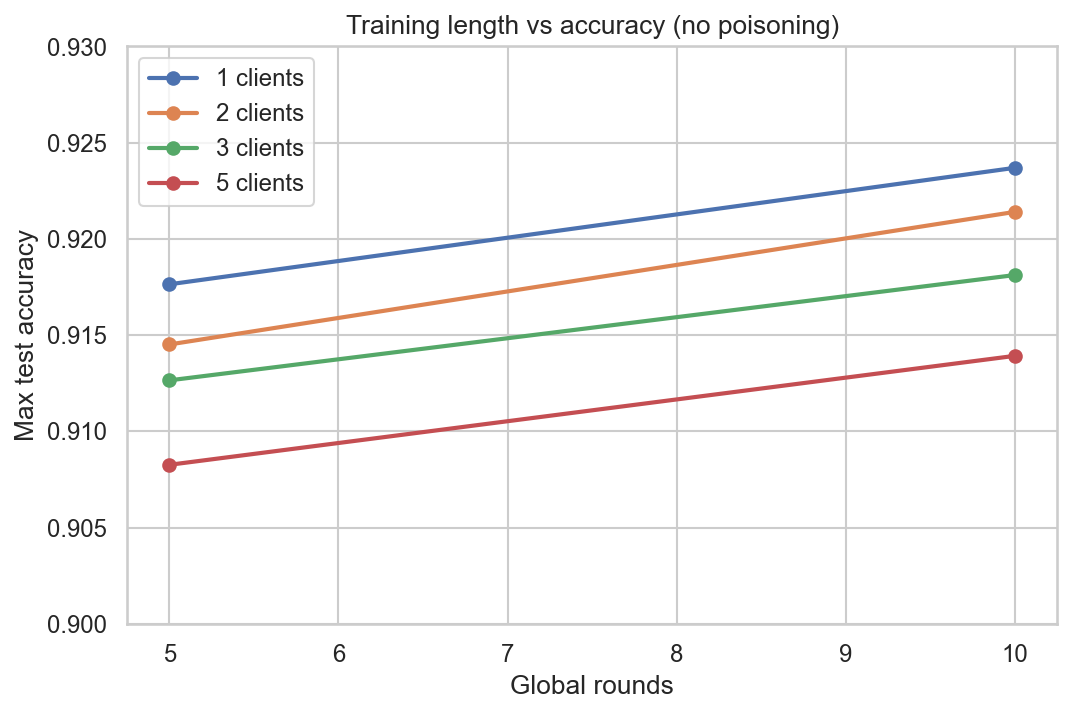
\includegraphics[width=\columnwidth]{03_rounds_vs_accuracy_clean.png}
\caption{Effect of global rounds on clean-run accuracy.}
\label{fig:rounds}
\end{figure}

\begin{figure}[!t]
\centering
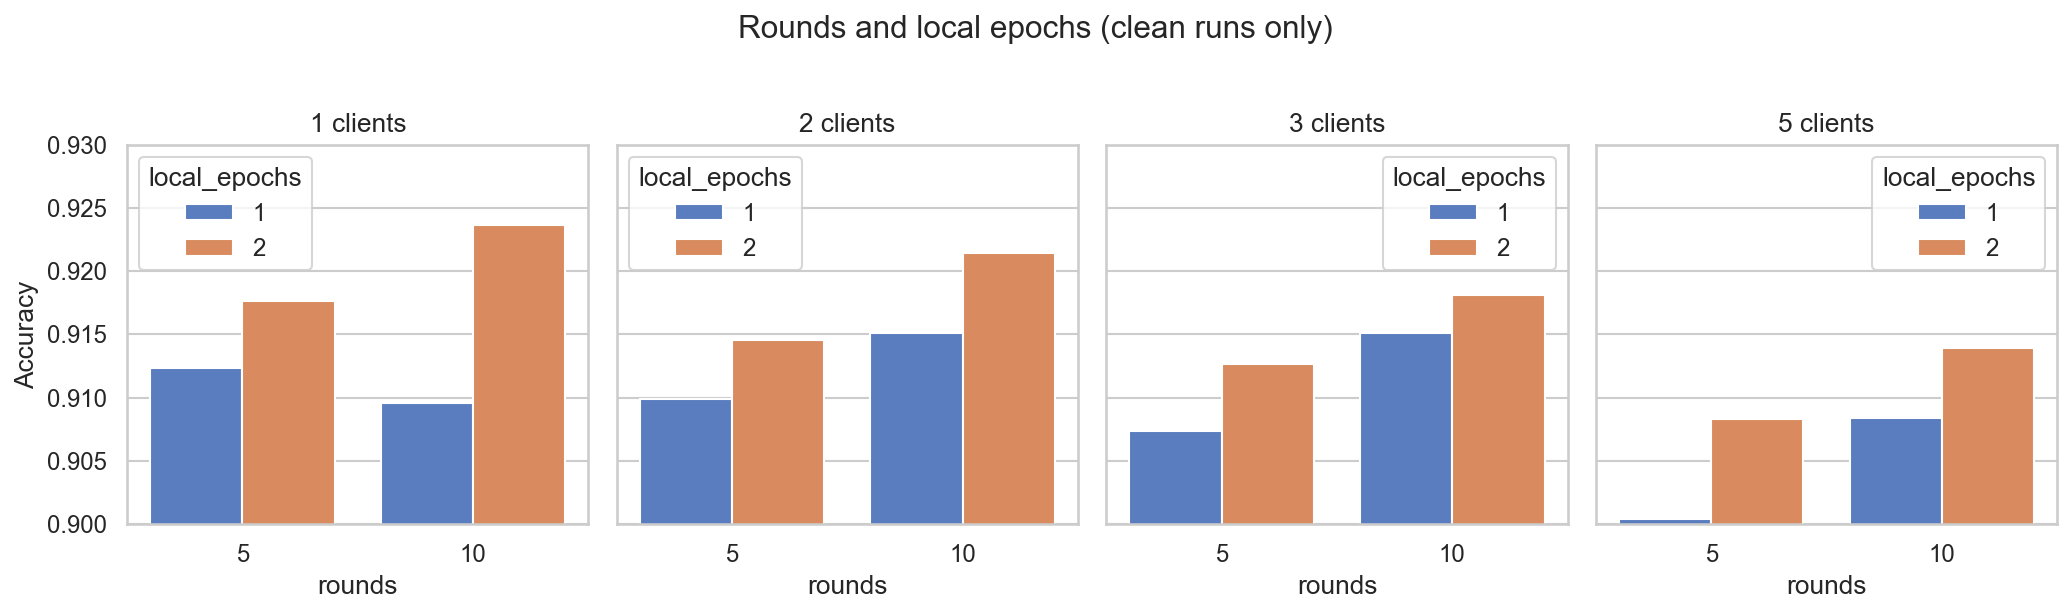
\includegraphics[width=\columnwidth]{06_local_epochs_clean_facets.png}
\caption{Local-epoch effects for clean federated runs.}
\label{fig:local_epochs}
\end{figure}

\subsection{Clients and Poison Scenarios}
Figure~\ref{fig:acc_scenario} compares best accuracy by client count and scenario. Figure~\ref{fig:heatmap} shows a clients-versus-poison heatmap of maximum accuracy. Figure~\ref{fig:clean_vs_poison} contrasts clean versus $40\%$ target poisoning.

\begin{figure}[!t]
\centering
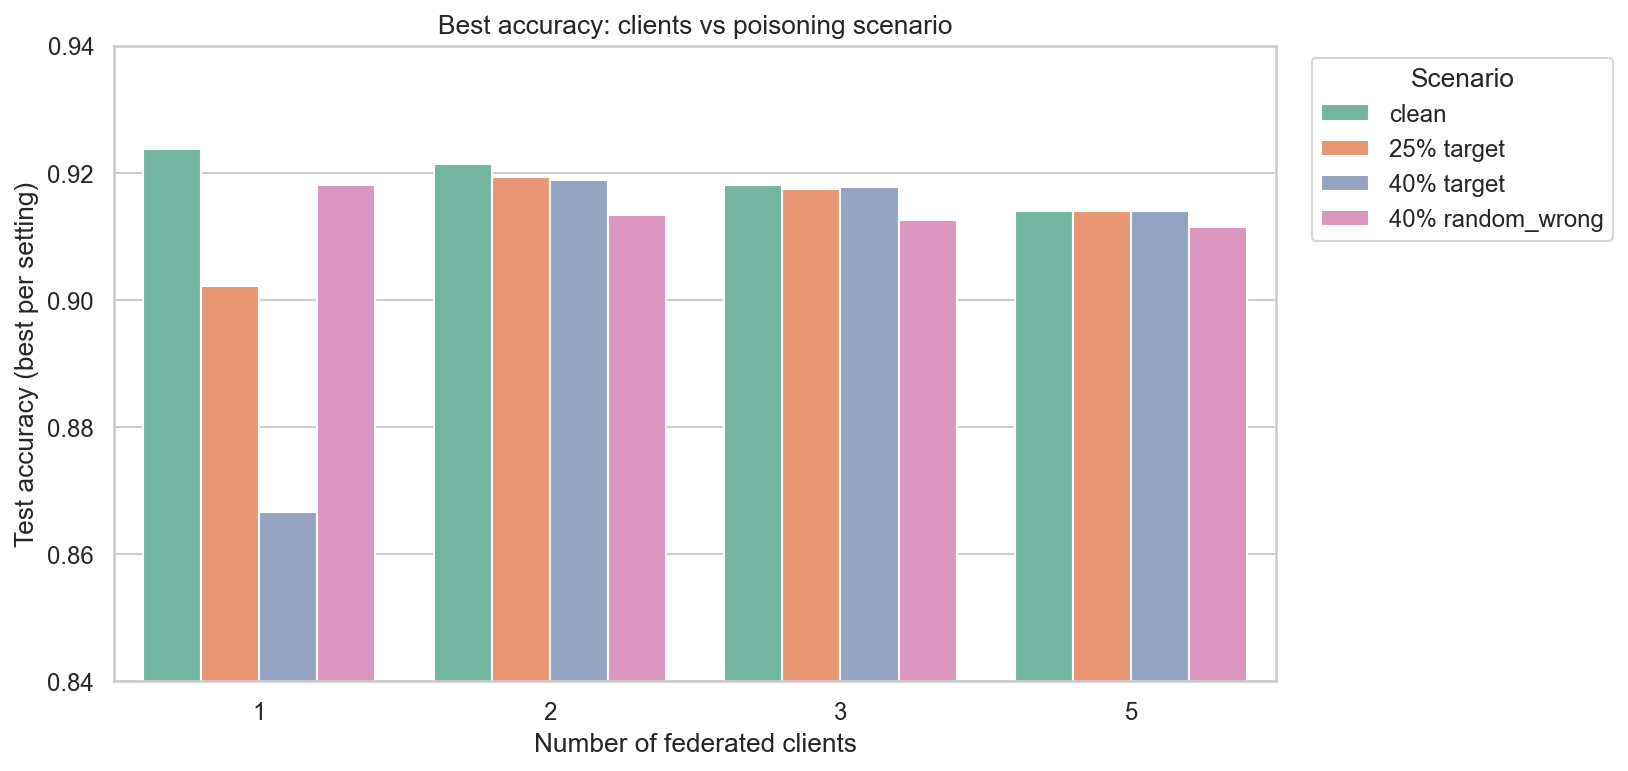
\includegraphics[width=\columnwidth]{01_accuracy_by_clients_scenario.png}
\caption{Best accuracy by client count and poisoning scenario.}
\label{fig:acc_scenario}
\end{figure}

\begin{figure}[!t]
\centering
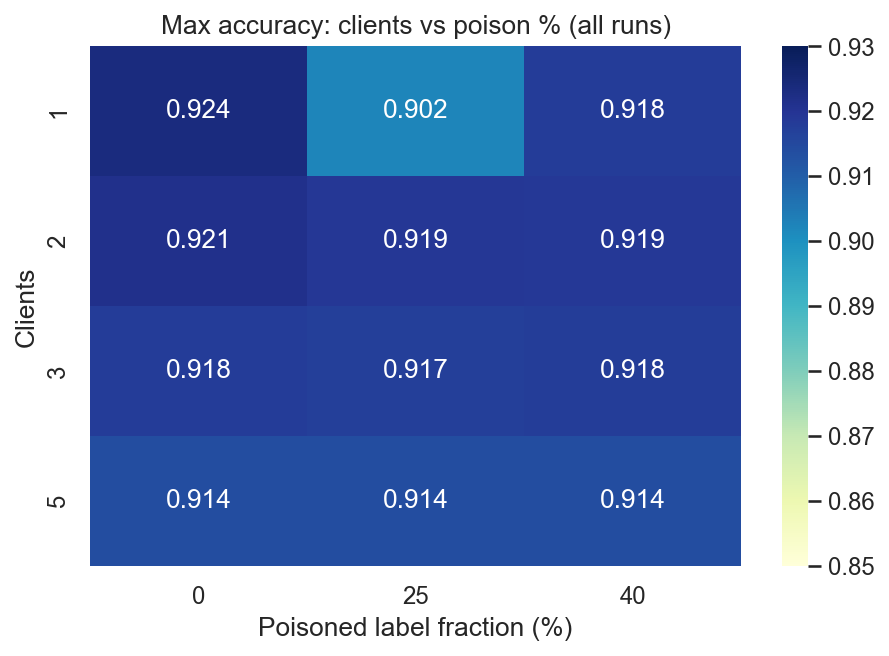
\includegraphics[width=\columnwidth]{02_heatmap_clients_poison_pct.png}
\caption{Max accuracy heatmap over clients versus poison percentage.}
\label{fig:heatmap}
\end{figure}

\begin{figure}[!t]
\centering
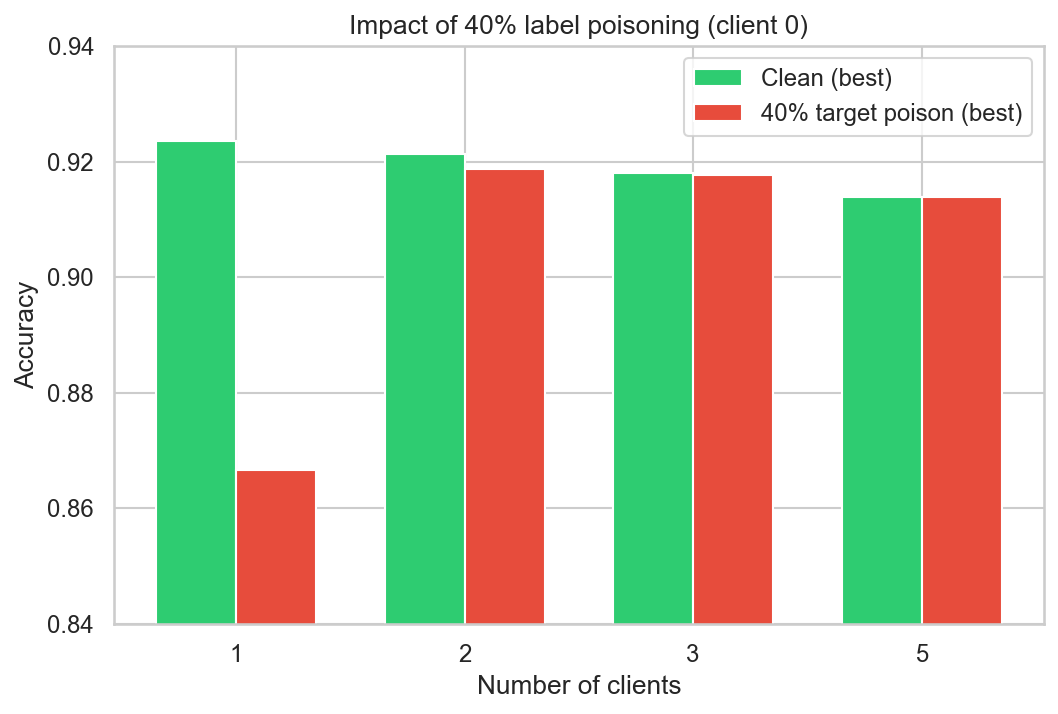
\includegraphics[width=\columnwidth]{04_clean_vs_40pct_target.png}
\caption{Clean versus $40\%$ target poisoning (best accuracy per client count).}
\label{fig:clean_vs_poison}
\end{figure}

\subsection{Best Configurations}
Table~\ref{tab:best} lists best observed metrics by condition. The most damaging cell is $N=1$ with $40\%$ target poison (accuracy $\approx 0.867$ in the best-of-condition table; some individual runs fall near $0.856$). By contrast, $N=5$ with $40\%$ target poison remains essentially tied with the clean five-client best ($\approx 0.914$).

\begin{table}[!t]
\caption{Best test accuracy by client count and poison setting}
\label{tab:best}
\centering
\renewcommand{\arraystretch}{1.15}
\begin{tabular}{ccccc}
\toprule
Clients & Poison & Mode & Acc. & F1 \\
\midrule
1 & 0\% & -- & 0.9237 & 0.9212 \\
1 & 25\% & target & 0.9022 & 0.8881 \\
1 & 40\% & target & 0.8666 & 0.8329 \\
1 & 40\% & random & 0.9180 & 0.9127 \\
2 & 0\% & -- & 0.9214 & 0.9177 \\
2 & 40\% & target & 0.9188 & 0.9132 \\
3 & 0\% & -- & 0.9181 & 0.9152 \\
3 & 40\% & target & 0.9178 & 0.9135 \\
5 & 0\% & -- & 0.9139 & 0.9119 \\
5 & 40\% & target & 0.9139 & 0.9117 \\
\bottomrule
\end{tabular}
\end{table}

\subsection{Mean Accuracy by Clients and Poison Fraction}
Table~\ref{tab:means} reports mean accuracy aggregated over rounds/epochs/modes in the sweep. The drop from $f=0$ to $f=0.4$ is large for $N=1$ ($\approx 0.916\to 0.887$ mean) and small for $N=5$ ($\approx 0.908\to 0.905$).

\begin{table}[!t]
\caption{Mean test accuracy by clients and poison fraction (sweep aggregate)}
\label{tab:means}
\centering
\begin{tabular}{cccc}
\toprule
Clients & $f=0$ & $f=0.25$ & $f=0.40$ \\
\midrule
1 & 0.9158 & 0.8981 & 0.8873 \\
2 & 0.9152 & 0.9141 & 0.9106 \\
3 & 0.9133 & 0.9127 & 0.9082 \\
5 & 0.9077 & 0.9076 & 0.9051 \\
\bottomrule
\end{tabular}
\end{table}

\subsection{Target versus Random-Wrong Poisoning}
Target poisoning toward class~0 is typically more harmful than random-wrong poisoning at the same fraction in low-$N$ regimes. Random-wrong noise is less coherently biased; target poisoning consistently teaches a majority-class prior. This distinction appears both in aggregate metrics and in confusion structure.

\subsection{Confusion Matrices: Clean Multi-Client}
Figures~\ref{fig:cm5c}--\ref{fig:cm5p} show five-client clean versus poisoned matrices. They are nearly alike: FedAvg dilution keeps decision boundaries stable. Class~0 dominates correct predictions; rare classes remain difficult; class~5 absorbs many off-diagonal errors.

\begin{figure}[!t]
\centering
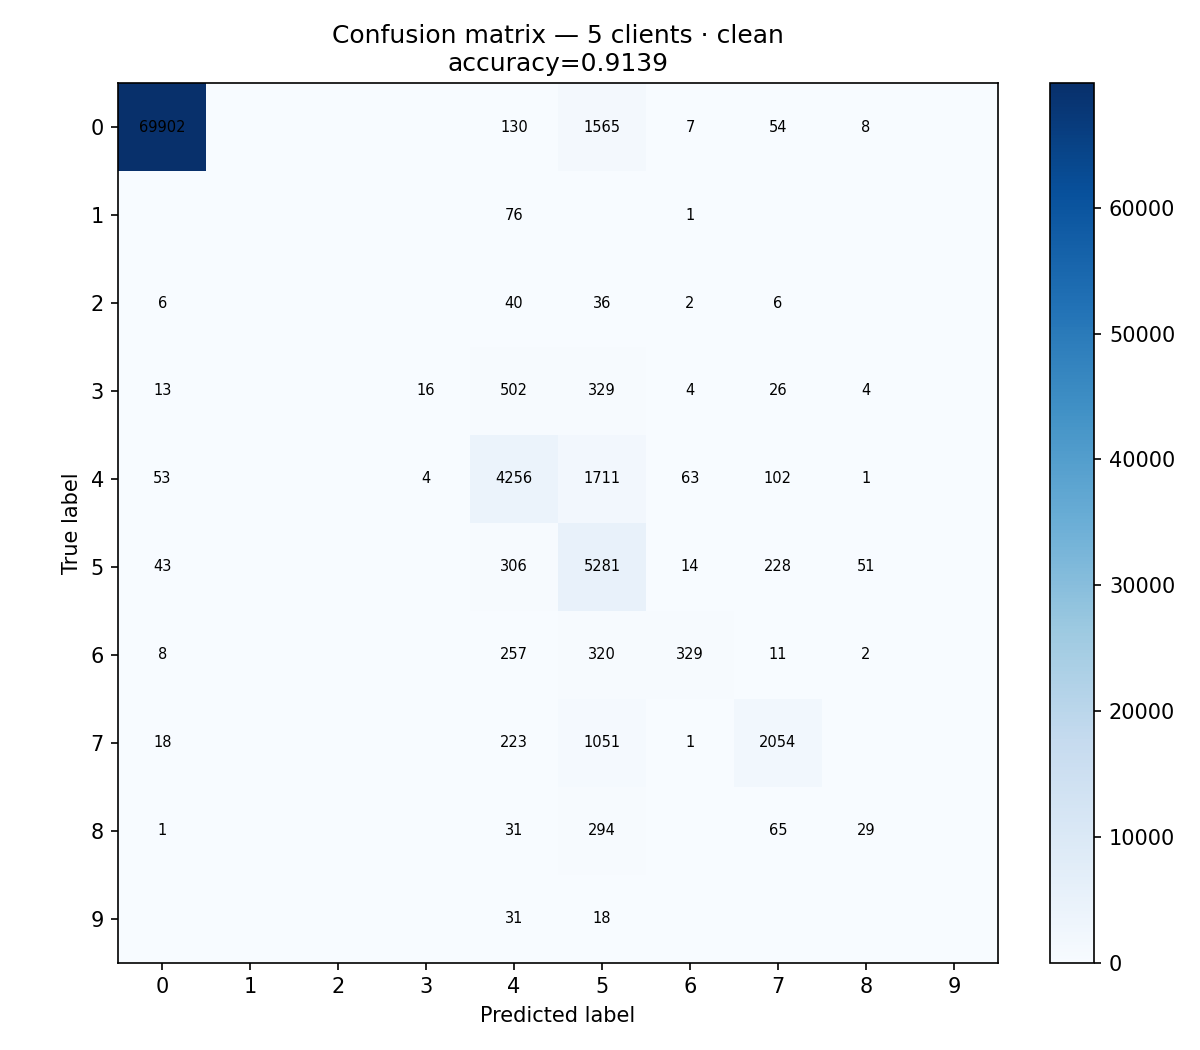
\includegraphics[width=\columnwidth]{cm_5_clients__clean.png}
\caption{Confusion matrix: 5 clients, clean training.}
\label{fig:cm5c}
\end{figure}

\begin{figure}[!t]
\centering
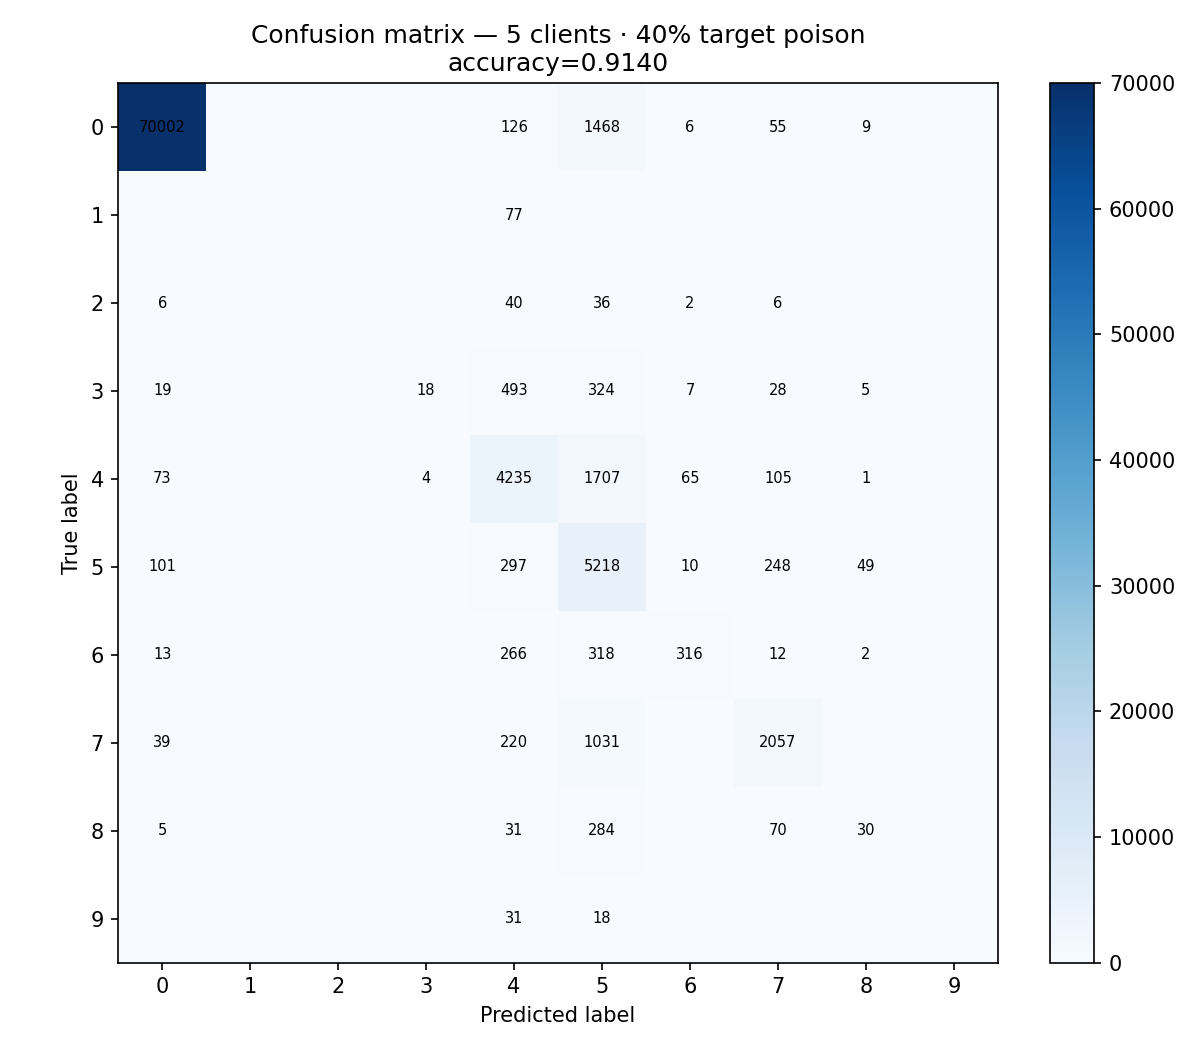
\includegraphics[width=\columnwidth]{cm_5_clients__40pct_target_poison.png}
\caption{Confusion matrix: 5 clients, $40\%$ target poison on client~0.}
\label{fig:cm5p}
\end{figure}

\subsection{Confusion Matrices: Single-Client Fragility}
Figures~\ref{fig:cm1c}--\ref{fig:cm1p} show the single-client contrast. After $40\%$ target poisoning, substantial mass moves into predicted class~0 from true classes 4, 5, 6, and 7. Class~0 recall can remain high or even increase, while other classes suffer. Figures~\ref{fig:tpfn_clean}--\ref{fig:tpfn_poison} make the same point via TP/FP/FN/TN bars: class~0 FP rises; FN rises for several non-zero classes.

\begin{figure}[!t]
\centering
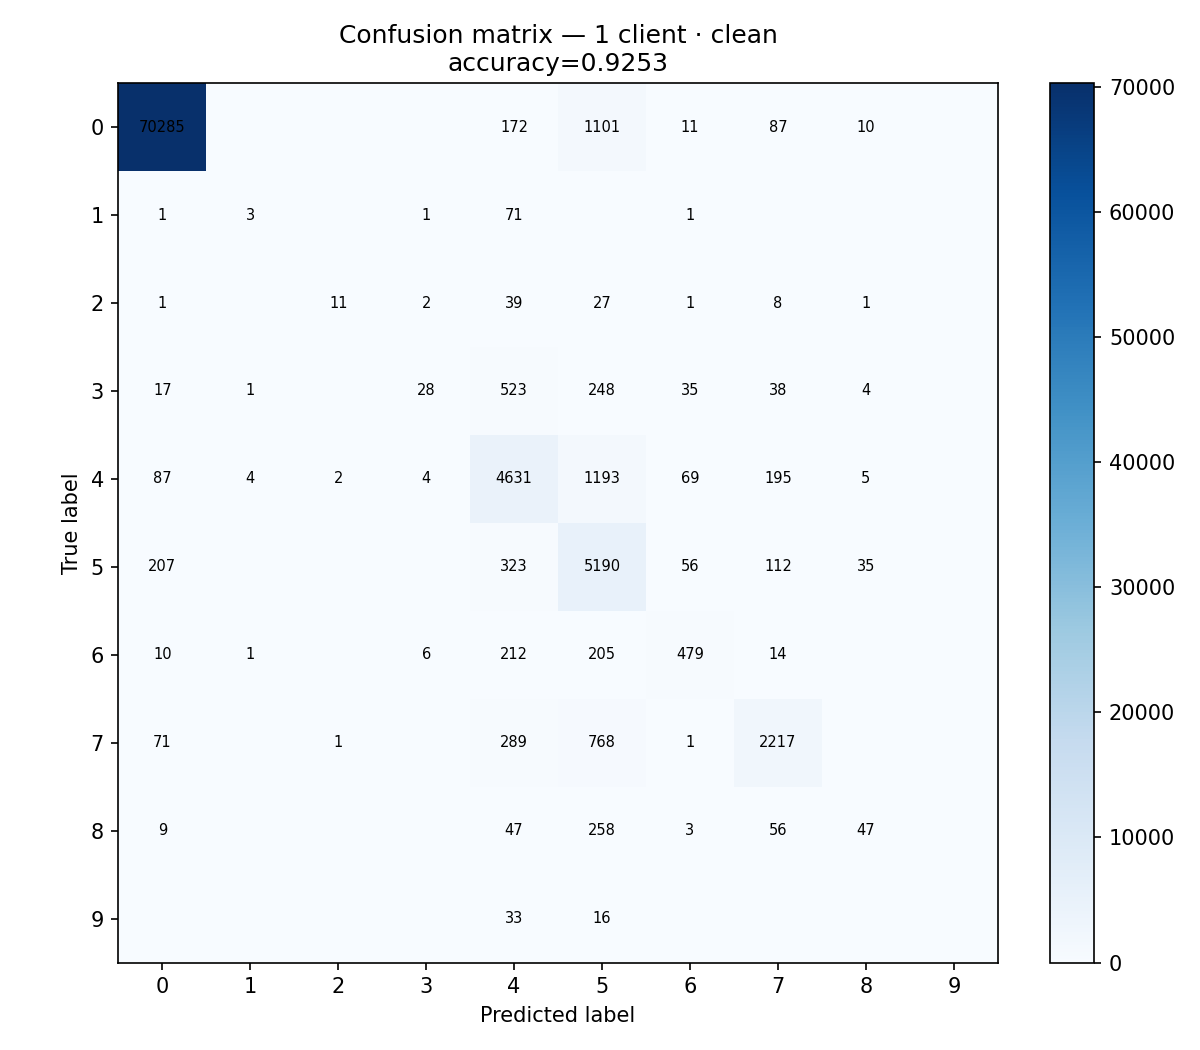
\includegraphics[width=\columnwidth]{cm_1_client__clean.png}
\caption{Confusion matrix: 1 client, clean training.}
\label{fig:cm1c}
\end{figure}

\begin{figure}[!t]
\centering
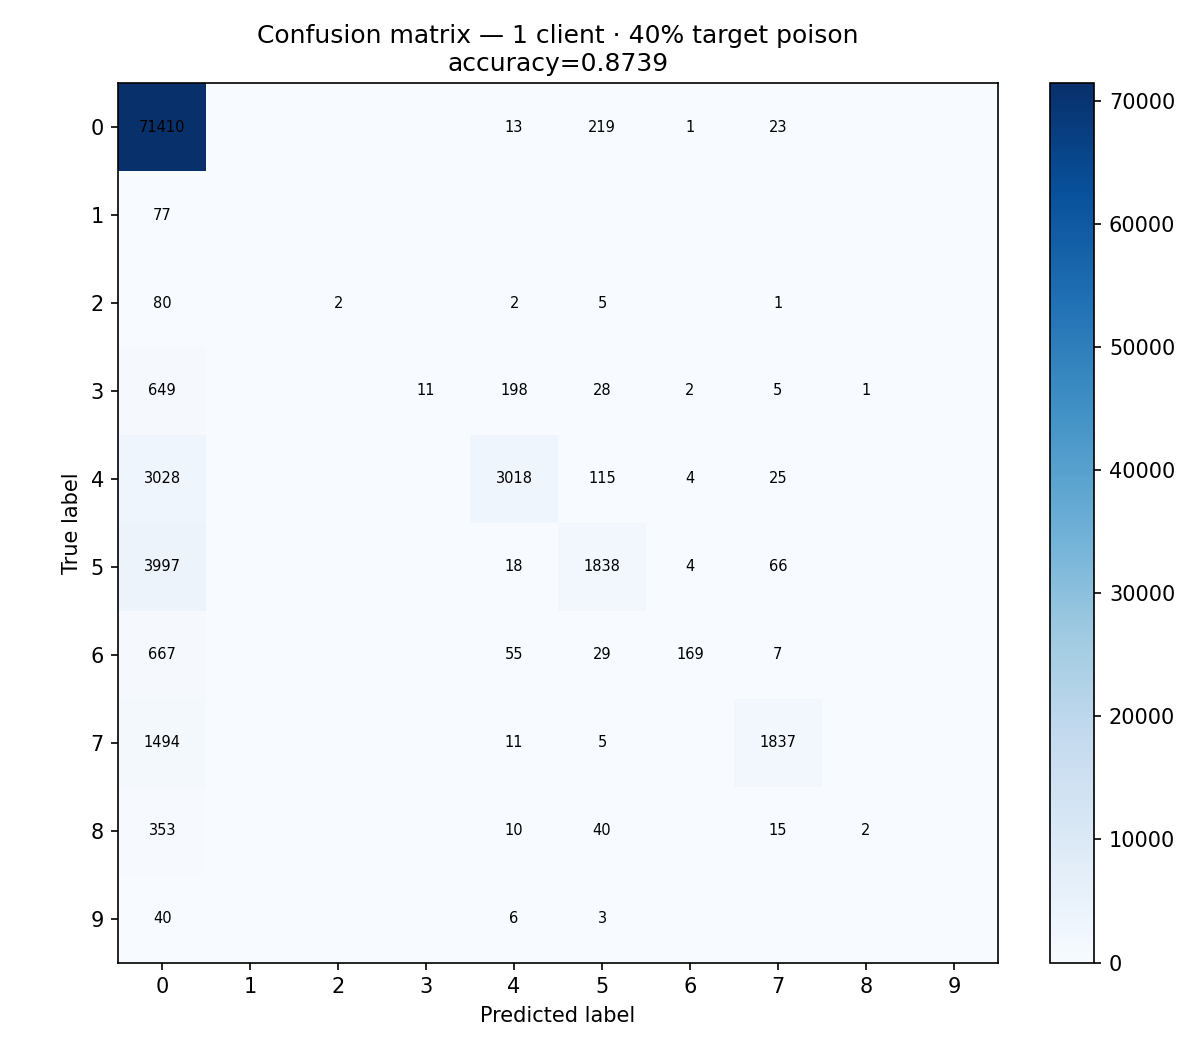
\includegraphics[width=\columnwidth]{cm_1_client__40pct_target_poison.png}
\caption{Confusion matrix: 1 client, $40\%$ target poison.}
\label{fig:cm1p}
\end{figure}

\begin{figure}[!t]
\centering
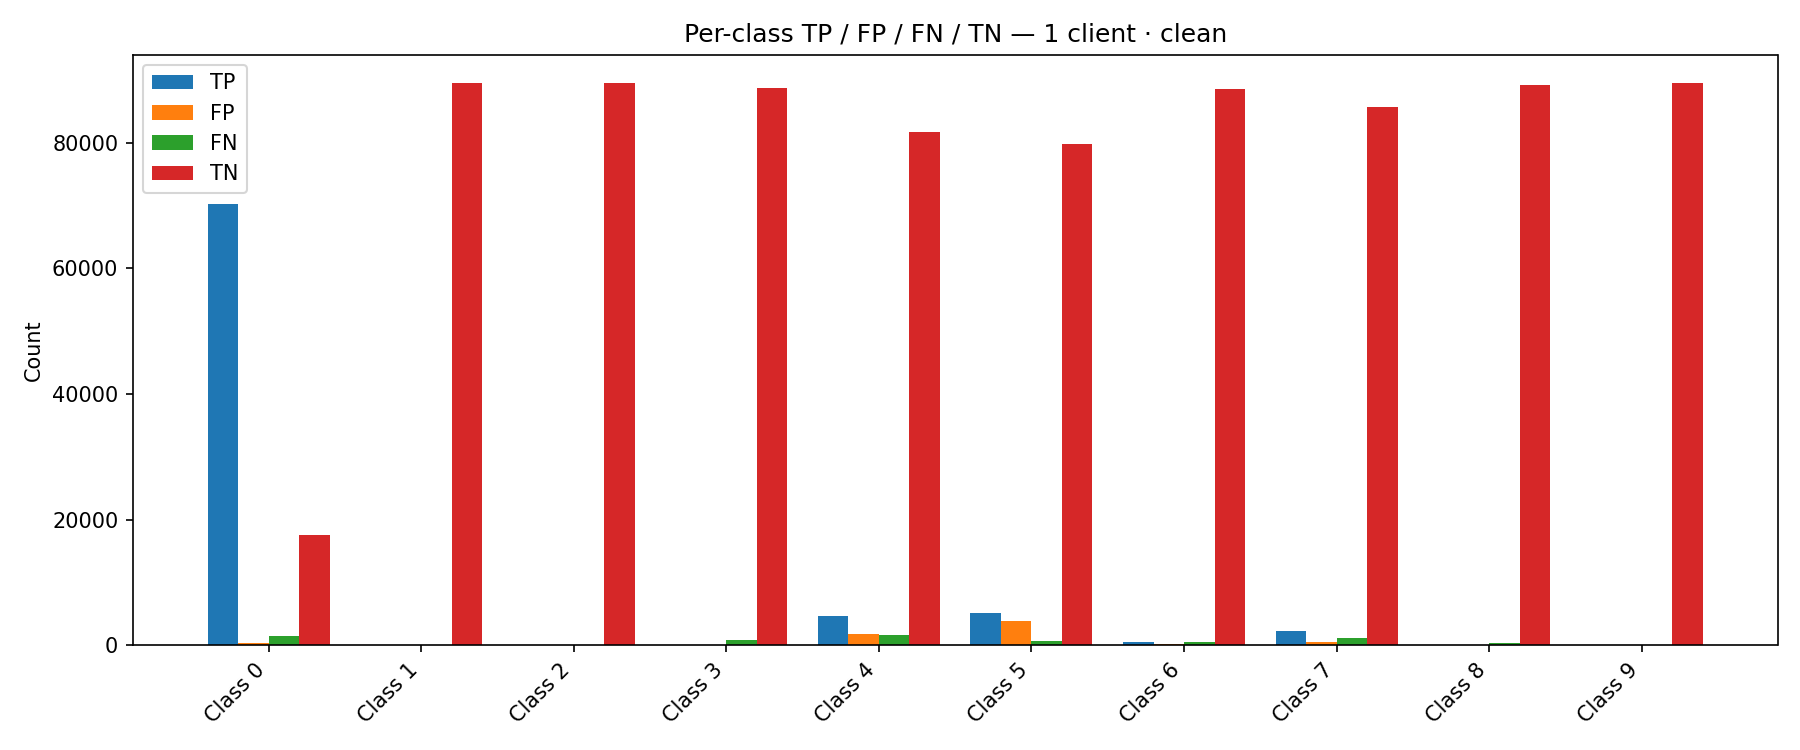
\includegraphics[width=\columnwidth]{tpfn_1_client__clean.png}
\caption{Per-class TP/FP/FN/TN: 1 client, clean.}
\label{fig:tpfn_clean}
\end{figure}

\begin{figure}[!t]
\centering
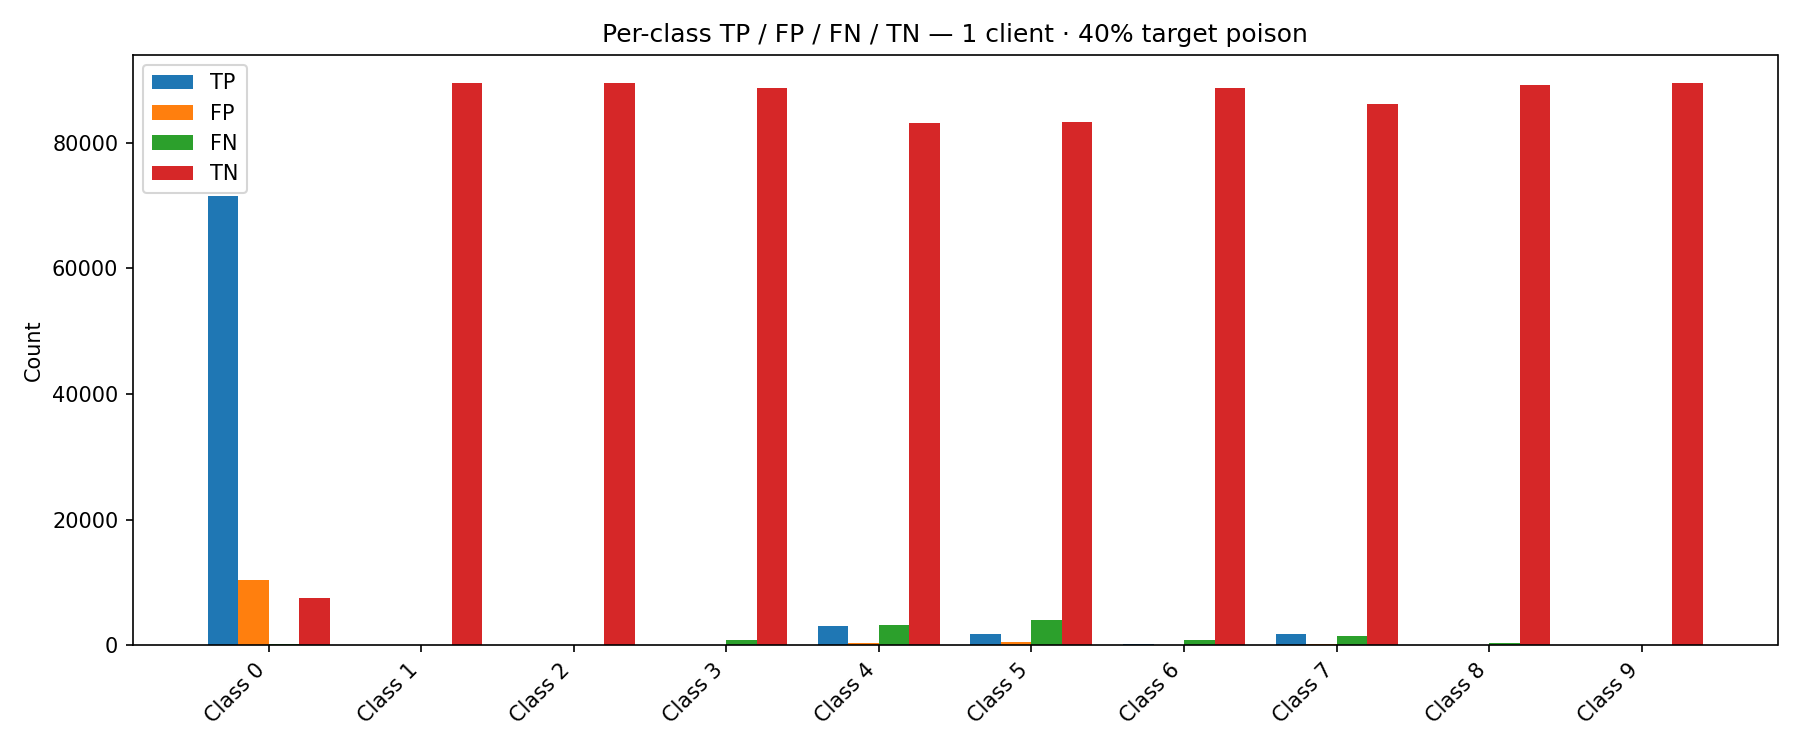
\includegraphics[width=\columnwidth]{tpfn_1_client__40pct_target_poison.png}
\caption{Per-class TP/FP/FN/TN: 1 client, $40\%$ target poison.}
\label{fig:tpfn_poison}
\end{figure}

\subsection{Security Interpretation of Errors}
From a SOC analyst's perspective, elevated class~0 false positives after target poisoning mean attack flows are more often declared ``majority/benign-like'' (depending on label semantics), i.e., \emph{missed detections}. Overall accuracy may still look acceptable because class~0 is frequent. This is why confusion-level reporting is mandatory for security ML evaluations.

\section{Discussion}
\label{sec:discussion}

\subsection{Implications for Deploying FL in IDS}
\begin{enumerate}
\item Prefer multiple independent data silos when possible; averaging provides baseline robustness to one bad silo under label noise.
\item Prefer adequate $R$ and $E$; under-trained models are both less accurate and potentially less stable under noise.
\item Monitor per-class recall, not only accuracy, especially for rare attack types.
\item Treat single-client ``federated'' training as essentially centralized: it inherits no dilution benefit.
\end{enumerate}

\subsection{What This Study Does Not Claim}
We do not claim FedAvg is secure against adaptive model-poisoning or colluding clients. We do not claim MLP is the optimal IDS architecture. We do not claim IID shards represent real institutional heterogeneity.

\subsection{Limitations}
\begin{itemize}
\item \textbf{IID simulation:} random shards underestimate heterogeneity-induced drift.
\item \textbf{Global scaler:} pooled normalization is a centralized shortcut.
\item \textbf{Single architecture:} no comparison to trees, CNNs on raw packets, or GNNs.
\item \textbf{Undefended aggregation:} no median/Krum/DP baselines.
\item \textbf{Label semantics:} class indices are used without exhaustive attack taxonomy narration.
\end{itemize}

\subsection{Threats to Validity}
Random seeds, hyperparameter choices (Adam lr, batch size), and the particular augmented dataset release could shift absolute numbers. Relative conclusions---dilution with $N$, severity of target poison at $N=1$, need for confusion analysis---were consistent across the sweep's internal variation.

\subsection{Future Work}
\begin{enumerate}
\item Non-IID label and feature skew across clients.
\item Robust aggregators and anomaly detection on updates.
\item Differentially private FL for formal privacy guarantees.
\item Cost-sensitive losses or resampling for rare classes.
\item Multi-poisoner and model-replacement attacks.
\item Deployment in a real FL framework with networked workers.
\end{enumerate}

\section{Conclusion}
\label{sec:conclusion}

We presented an expanded theoretical and experimental study of FedAvg for multi-class traffic classification on CIC--UNSW-NB15. Starting from the global empirical risk and its client-wise decomposition, we formalized local optimization, size-weighted aggregation, communication scaling, class-imbalance metrics, and a single-client label-poisoning adversary. Empirically, among 64 configurations, clean training benefits from more rounds and local epochs; targeted poisoning is highly damaging when $N=1$ and largely diluted when $N\ge 2$; and confusion matrices reveal majority-class bias that accuracy can mask. These findings support a practical message: federated collaboration with multiple honest clients, sufficient training, and per-class monitoring forms a stronger baseline than accuracy-only evaluation of single-silo training under label noise.

\section*{Acknowledgment}
The author thanks the maintainers of CIC--UNSW-NB15 related public datasets and the developers of PyTorch, NumPy, pandas, and scikit-learn.

\begin{thebibliography}{00}
\bibitem{mcmahan2017communication}
H.~B. McMahan, E.~Moore, D.~Ramage, S.~Hampson, and B.~A. y~Arcas,
``Communication-efficient learning of deep networks from decentralized data,''
in \emph{Proc. AISTATS}, 2017, pp. 1273--1282.

\bibitem{kairouz2021advances}
P.~Kairouz \textit{et al.},
``Advances and open problems in federated learning,''
\emph{Found. Trends Mach. Learn.}, vol.~14, no.~1--2, pp. 1--210, 2021.

\bibitem{rahman2020internet}
S.~A. Rahman, H.~Tout, C.~Talhi, and A.~Mourad,
``Internet of Things intrusion detection: Centralized, on-device, or federated learning?''
\emph{IEEE Network}, vol.~34, no.~6, pp. 310--317, 2020.

\bibitem{bagdasaryan2020backdoor}
E.~Bagdasaryan, A.~Veit, Y.~Hua, D.~Estrin, and V.~Shmatikov,
``How to backdoor federated learning,''
in \emph{Proc. AISTATS}, 2020, pp. 2938--2948.

\bibitem{tolpegin2020data}
V.~Tolpegin, S.~Truex, M.~E. Gursoy, and L.~Liu,
``Data poisoning attacks against federated learning systems,''
in \emph{Proc. ESORICS}, 2020, pp. 480--501.

\bibitem{li2020federated}
T.~Li, A.~K. Sahu, A.~Talwalkar, and V.~Smith,
``Federated learning: Challenges, methods, and future directions,''
\emph{IEEE Signal Process. Mag.}, vol.~37, no.~3, pp. 50--60, 2020.

\bibitem{bonawitz2019towards}
K.~Bonawitz \textit{et al.},
``Towards federated learning at scale: System design,''
in \emph{Proc. MLSys}, 2019.

\bibitem{moustafa2015unsw}
N.~Moustafa and J.~Slay,
``UNSW-NB15: A comprehensive data set for network intrusion detection systems,''
in \emph{Proc. MilCIS}, 2015, pp. 1--6.

\bibitem{blanchard2017machine}
P.~Blanchard, E.~M. El~Mhamdi, R.~Guerraoui, and J.~Stainer,
``Machine learning with adversaries: Byzantine tolerant gradient descent,''
in \emph{Proc. NeurIPS}, 2017.

\bibitem{yin2018byzantine}
D.~Yin, Y.~Chen, R.~Kannan, and P.~Bartlett,
``Byzantine-robust distributed learning: Towards optimal statistical rates,''
in \emph{Proc. ICML}, 2018.
\end{thebibliography}

\end{document}
